\documentclass[twoside]{book}

% Packages required by doxygen
\usepackage{fixltx2e}
\usepackage{calc}
\usepackage{doxygen}
\usepackage[export]{adjustbox} % also loads graphicx
\usepackage{graphicx}
\usepackage[utf8]{inputenc}
\usepackage{makeidx}
\usepackage{multicol}
\usepackage{multirow}
\PassOptionsToPackage{warn}{textcomp}
\usepackage{textcomp}
\usepackage[nointegrals]{wasysym}
\usepackage[table]{xcolor}

% Font selection
\usepackage[T1]{fontenc}
\usepackage[scaled=.90]{helvet}
\usepackage{courier}
\usepackage{amssymb}
\usepackage{sectsty}
\renewcommand{\familydefault}{\sfdefault}
\allsectionsfont{%
  \fontseries{bc}\selectfont%
  \color{darkgray}%
}
\renewcommand{\DoxyLabelFont}{%
  \fontseries{bc}\selectfont%
  \color{darkgray}%
}
\newcommand{\+}{\discretionary{\mbox{\scriptsize$\hookleftarrow$}}{}{}}

% Page & text layout
\usepackage{geometry}
\geometry{%
  a4paper,%
  top=2.5cm,%
  bottom=2.5cm,%
  left=2.5cm,%
  right=2.5cm%
}
\tolerance=750
\hfuzz=15pt
\hbadness=750
\setlength{\emergencystretch}{15pt}
\setlength{\parindent}{0cm}
\setlength{\parskip}{3ex plus 2ex minus 2ex}
\makeatletter
\renewcommand{\paragraph}{%
  \@startsection{paragraph}{4}{0ex}{-1.0ex}{1.0ex}{%
    \normalfont\normalsize\bfseries\SS@parafont%
  }%
}
\renewcommand{\subparagraph}{%
  \@startsection{subparagraph}{5}{0ex}{-1.0ex}{1.0ex}{%
    \normalfont\normalsize\bfseries\SS@subparafont%
  }%
}
\makeatother

% Headers & footers
\usepackage{fancyhdr}
\pagestyle{fancyplain}
\fancyhead[LE]{\fancyplain{}{\bfseries\thepage}}
\fancyhead[CE]{\fancyplain{}{}}
\fancyhead[RE]{\fancyplain{}{\bfseries\leftmark}}
\fancyhead[LO]{\fancyplain{}{\bfseries\rightmark}}
\fancyhead[CO]{\fancyplain{}{}}
\fancyhead[RO]{\fancyplain{}{\bfseries\thepage}}
\fancyfoot[LE]{\fancyplain{}{}}
\fancyfoot[CE]{\fancyplain{}{}}
\fancyfoot[RE]{\fancyplain{}{\bfseries\scriptsize Generated by Doxygen }}
\fancyfoot[LO]{\fancyplain{}{\bfseries\scriptsize Generated by Doxygen }}
\fancyfoot[CO]{\fancyplain{}{}}
\fancyfoot[RO]{\fancyplain{}{}}
\renewcommand{\footrulewidth}{0.4pt}
\renewcommand{\chaptermark}[1]{%
  \markboth{#1}{}%
}
\renewcommand{\sectionmark}[1]{%
  \markright{\thesection\ #1}%
}

% Indices & bibliography
\usepackage{natbib}
\usepackage[titles]{tocloft}
\setcounter{tocdepth}{3}
\setcounter{secnumdepth}{5}
\makeindex

% Hyperlinks (required, but should be loaded last)
\usepackage{ifpdf}
\ifpdf
  \usepackage[pdftex,pagebackref=true]{hyperref}
\else
  \usepackage[ps2pdf,pagebackref=true]{hyperref}
\fi
\hypersetup{%
  colorlinks=true,%
  linkcolor=blue,%
  citecolor=blue,%
  unicode%
}

% Custom commands
\newcommand{\clearemptydoublepage}{%
  \newpage{\pagestyle{empty}\cleardoublepage}%
}

\usepackage{caption}
\captionsetup{labelsep=space,justification=centering,font={bf},singlelinecheck=off,skip=4pt,position=top}

%===== C O N T E N T S =====

\begin{document}

% Titlepage & ToC
\hypersetup{pageanchor=false,
             bookmarksnumbered=true,
             pdfencoding=unicode
            }
\pagenumbering{alph}
\begin{titlepage}
\vspace*{7cm}
\begin{center}%
{\Large Piloop \\[1ex]\large 0.\+3 }\\
\vspace*{1cm}
{\large Generated by Doxygen 1.8.14}\\
\end{center}
\end{titlepage}
\clearemptydoublepage
\pagenumbering{roman}
\tableofcontents
\clearemptydoublepage
\pagenumbering{arabic}
\hypersetup{pageanchor=true}

%--- Begin generated contents ---
\chapter{Hierarchical Index}
\section{Class Hierarchy}
This inheritance list is sorted roughly, but not completely, alphabetically\+:\begin{DoxyCompactList}
\item \contentsline{section}{channel}{\pageref{classchannel}}{}
\item \contentsline{section}{handshake}{\pageref{classhandshake}}{}
\item \contentsline{section}{route}{\pageref{classroute}}{}
\begin{DoxyCompactList}
\item \contentsline{section}{audiotrack}{\pageref{classaudiotrack}}{}
\item \contentsline{section}{miditrack}{\pageref{classmiditrack}}{}
\end{DoxyCompactList}
\item \contentsline{section}{session}{\pageref{classsession}}{}
\item \contentsline{section}{track}{\pageref{classtrack}}{}
\item \contentsline{section}{track\+\_\+port}{\pageref{structtrack__port}}{}
\end{DoxyCompactList}

\chapter{Class Index}
\doxysection{Class List}
Here are the classes, structs, unions and interfaces with brief descriptions\+:\begin{DoxyCompactList}
\item\contentsline{section}{\mbox{\hyperlink{classAudioServer}{Audio\+Server}} \\*The jack-\/audio server running on the alsa drivers }{\pageref{classAudioServer}}{}
\item\contentsline{section}{\mbox{\hyperlink{classButtons}{Buttons}} \\*\mbox{\hyperlink{classButtons}{Buttons}} as the G\+P\+I\+O-\/based input interface }{\pageref{classButtons}}{}
\item\contentsline{section}{\mbox{\hyperlink{classChannel}{Channel}} \\*Defines a looper-\/channel designed to loop tracks }{\pageref{classChannel}}{}
\item\contentsline{section}{\mbox{\hyperlink{classConfig}{Config}} \\*The config module responsible for saving, loading, and initializing session data }{\pageref{classConfig}}{}
\item\contentsline{section}{\mbox{\hyperlink{classEffects}{Effects}} \\*The effects module. Currently unsupported }{\pageref{classEffects}}{}
\item\contentsline{section}{\mbox{\hyperlink{classHandshake}{Handshake}} \\*The jack-\/audio client }{\pageref{classHandshake}}{}
\item\contentsline{section}{\mbox{\hyperlink{classhardwareInterface}{hardware\+Interface}} \\*The generic interface of the pi-\/loop. It has an input and an output interface }{\pageref{classhardwareInterface}}{}
\item\contentsline{section}{\mbox{\hyperlink{classKeyboard}{Keyboard}} \\*The keyboard as the computer-\/based input interface }{\pageref{classKeyboard}}{}
\item\contentsline{section}{\mbox{\hyperlink{classLeds}{Leds}} \\*L\+E\+Ds as the G\+P\+I\+O-\/based output interface }{\pageref{classLeds}}{}
\item\contentsline{section}{\mbox{\hyperlink{classLooper}{Looper}} \\*Constisted of 3 loop-\/channels }{\pageref{classLooper}}{}
\item\contentsline{section}{\mbox{\hyperlink{structLooperState}{Looper\+State}} \\*Stores the looper state }{\pageref{structLooperState}}{}
\item\contentsline{section}{\mbox{\hyperlink{classMenu}{Menu}} \\*The programs menu that acts as the session manager }{\pageref{classMenu}}{}
\item\contentsline{section}{\mbox{\hyperlink{classMetronome}{Metronome}} \\*A metronome defined within \mbox{\hyperlink{classLooper}{Looper}} }{\pageref{classMetronome}}{}
\item\contentsline{section}{\mbox{\hyperlink{classMixer}{Mixer}} \\*The mixer module responsible to stream the output signal }{\pageref{classMixer}}{}
\item\contentsline{section}{\mbox{\hyperlink{classMonitor}{Monitor}} \\*The monitor module encapsulates the jack audio client }{\pageref{classMonitor}}{}
\item\contentsline{section}{\mbox{\hyperlink{classPiLoop}{Pi\+Loop}} \\*The threading manager. It starts the program }{\pageref{classPiLoop}}{}
\item\contentsline{section}{\mbox{\hyperlink{classPotentiometers}{Potentiometers}} \\*\mbox{\hyperlink{classPotentiometers}{Potentiometers}} to adjust the looper-\/channel\textquotesingle{}s volume }{\pageref{classPotentiometers}}{}
\item\contentsline{section}{\mbox{\hyperlink{structResponse}{Response}} \\*Defines a response message destinated to the displayer module of the program }{\pageref{structResponse}}{}
\item\contentsline{section}{\mbox{\hyperlink{classScreen}{Screen}} \\*The screen as the computer-\/based output interface }{\pageref{classScreen}}{}
\item\contentsline{section}{\mbox{\hyperlink{classSession}{Session}} \\*Defines a musical session. It is consisted of a \mbox{\hyperlink{classMonitor}{Monitor}}, a \mbox{\hyperlink{classLooper}{Looper}} and a \mbox{\hyperlink{classMixer}{Mixer}} }{\pageref{classSession}}{}
\item\contentsline{section}{\mbox{\hyperlink{structtime__signature}{time\+\_\+signature}} \\*Struct to hold the information of rythm }{\pageref{structtime__signature}}{}
\item\contentsline{section}{\mbox{\hyperlink{structTrigger}{Trigger}} \\*Holds the triggers of the user }{\pageref{structTrigger}}{}
\item\contentsline{section}{\mbox{\hyperlink{classUI}{UI}} \\*Defines a computer based interface constisted of a keyboard and the screen }{\pageref{classUI}}{}
\end{DoxyCompactList}

\chapter{Class Documentation}
\hypertarget{classaudiotrack}{}\section{audiotrack Class Reference}
\label{classaudiotrack}\index{audiotrack@{audiotrack}}
Inheritance diagram for audiotrack\+:\begin{figure}[H]
\begin{center}
\leavevmode
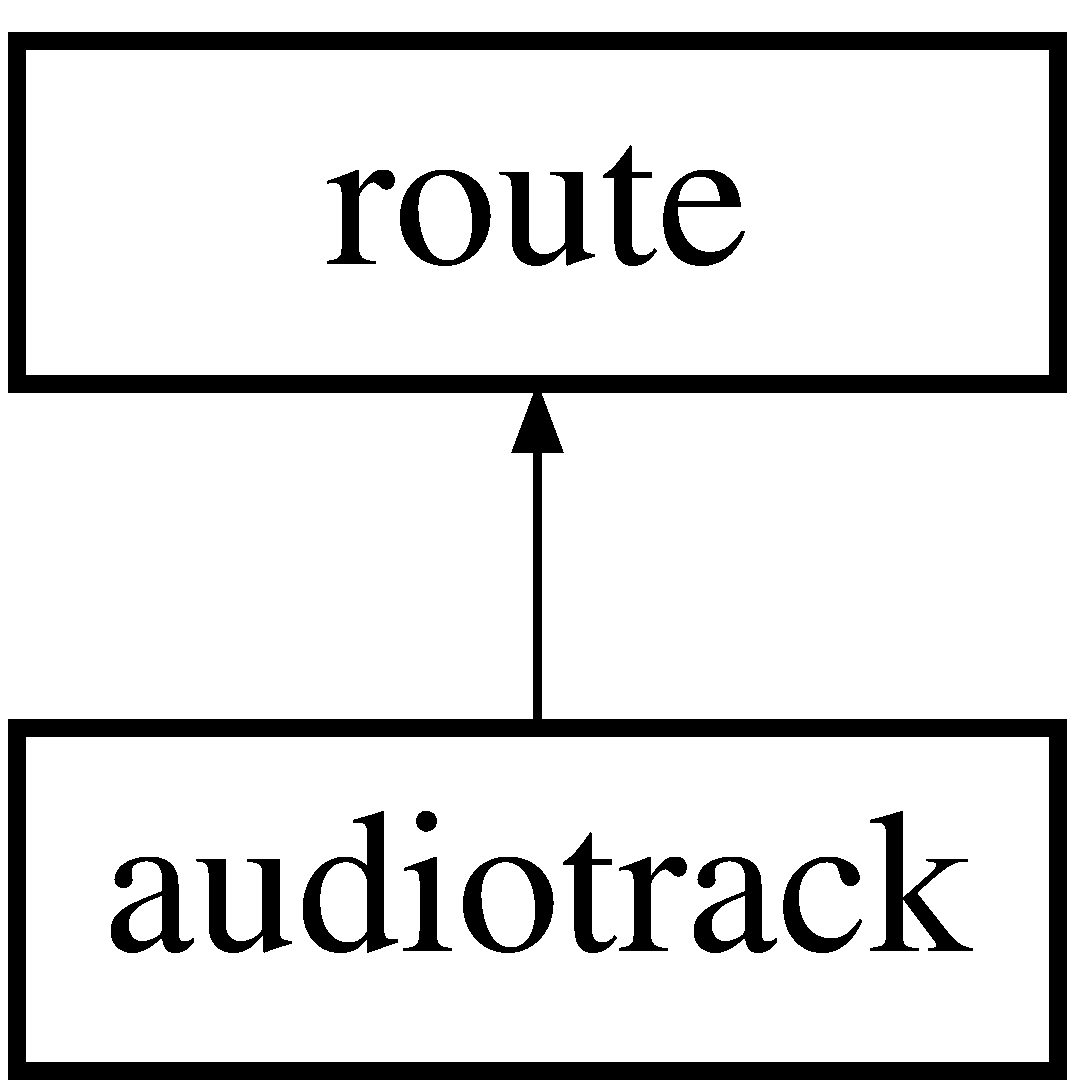
\includegraphics[height=2.000000cm]{classaudiotrack}
\end{center}
\end{figure}
\subsection*{Additional Inherited Members}


The documentation for this class was generated from the following files\+:\begin{DoxyCompactItemize}
\item 
src/audiotrack.\+h\item 
src/audiotrack.\+cpp\end{DoxyCompactItemize}

\hypertarget{classchannel}{}\section{channel Class Reference}
\label{classchannel}\index{channel@{channel}}
\subsection*{Public Member Functions}
\begin{DoxyCompactItemize}
\item 
\mbox{\Hypertarget{classchannel_a130a2f64e5d4d2bbebf5cca1f572cd98}\label{classchannel_a130a2f64e5d4d2bbebf5cca1f572cd98}} 
int {\bfseries monitor} (uint32\+\_\+t nframes)
\item 
\mbox{\Hypertarget{classchannel_ad290679ac4562b61e29dad7e2ee6afe5}\label{classchannel_ad290679ac4562b61e29dad7e2ee6afe5}} 
void {\bfseries mute\+\_\+monitor} ()
\item 
\mbox{\Hypertarget{classchannel_a80fe57d86e13a757b4da322fb58f10e8}\label{classchannel_a80fe57d86e13a757b4da322fb58f10e8}} 
void {\bfseries unmute\+\_\+monitor} ()
\item 
\mbox{\Hypertarget{classchannel_a89108f9e9c8722c694794812441976dd}\label{classchannel_a89108f9e9c8722c694794812441976dd}} 
void {\bfseries mute\+\_\+channel} ()
\item 
\mbox{\Hypertarget{classchannel_af6a2f423b995869b2ec0a2265f32f907}\label{classchannel_af6a2f423b995869b2ec0a2265f32f907}} 
void {\bfseries unmute\+\_\+channel} ()
\item 
\mbox{\Hypertarget{classchannel_aa87ebcc47bdf707ef59653b6c78f65b9}\label{classchannel_aa87ebcc47bdf707ef59653b6c78f65b9}} 
void {\bfseries record} ()
\item 
\mbox{\Hypertarget{classchannel_a3ac3a6cf05b4e8a5b5884a10b8a6c0a4}\label{classchannel_a3ac3a6cf05b4e8a5b5884a10b8a6c0a4}} 
void {\bfseries stop} ()
\item 
\mbox{\Hypertarget{classchannel_afd7ccbda42c0ede6c84098a97783b9a2}\label{classchannel_afd7ccbda42c0ede6c84098a97783b9a2}} 
void {\bfseries playback} ()
\item 
\mbox{\Hypertarget{classchannel_ad7efc911726f155af8df17004d7962fc}\label{classchannel_ad7efc911726f155af8df17004d7962fc}} 
void {\bfseries undo} ()
\item 
\mbox{\Hypertarget{classchannel_acdd44b1676fb73669d06ce94079f04eb}\label{classchannel_acdd44b1676fb73669d06ce94079f04eb}} 
void {\bfseries disconnect\+\_\+channel} ()
\item 
\mbox{\Hypertarget{classchannel_a04ea6b0dd5037b24ea8f7fe983fd6ad9}\label{classchannel_a04ea6b0dd5037b24ea8f7fe983fd6ad9}} 
\mbox{\hyperlink{classhandshake}{handshake}} $\ast$ {\bfseries get\+\_\+\+IO} ()
\end{DoxyCompactItemize}


The documentation for this class was generated from the following files\+:\begin{DoxyCompactItemize}
\item 
src/channel.\+h\item 
src/channel.\+cpp\end{DoxyCompactItemize}

\hypertarget{classhandshake}{}\section{handshake Class Reference}
\label{classhandshake}\index{handshake@{handshake}}
\subsection*{Public Member Functions}
\begin{DoxyCompactItemize}
\item 
\mbox{\Hypertarget{classhandshake_aec0b12c760a648e1b4fc40be11529a21}\label{classhandshake_aec0b12c760a648e1b4fc40be11529a21}} 
{\bfseries handshake} (const char $\ast$clientname)
\item 
\mbox{\Hypertarget{classhandshake_a1229342aa52da4b1d480d4791311b9d2}\label{classhandshake_a1229342aa52da4b1d480d4791311b9d2}} 
jack\+\_\+client\+\_\+t $\ast$ {\bfseries get\+\_\+client} ()
\item 
\mbox{\Hypertarget{classhandshake_af0ce8d96a76d8b157c73d40d4e5330de}\label{classhandshake_af0ce8d96a76d8b157c73d40d4e5330de}} 
jack\+\_\+port\+\_\+t $\ast$ {\bfseries add\+\_\+input\+\_\+port} (jack\+\_\+port\+\_\+t $\ast$\+\_\+port, const char $\ast$inport\+\_\+name)
\item 
\mbox{\Hypertarget{classhandshake_aa227451908beaa17890b582eda2d59f5}\label{classhandshake_aa227451908beaa17890b582eda2d59f5}} 
jack\+\_\+port\+\_\+t $\ast$ {\bfseries add\+\_\+output\+\_\+port} (jack\+\_\+port\+\_\+t $\ast$\+\_\+port, const char $\ast$outport\+\_\+name)
\item 
\mbox{\Hypertarget{classhandshake_a915e38ef7fe8687a3fc27b3a91986297}\label{classhandshake_a915e38ef7fe8687a3fc27b3a91986297}} 
void {\bfseries disconnect\+\_\+port} (jack\+\_\+port\+\_\+t $\ast$\+\_\+port)
\item 
\mbox{\Hypertarget{classhandshake_a43d9fa50a21d39605ff67c1ab875ce2d}\label{classhandshake_a43d9fa50a21d39605ff67c1ab875ce2d}} 
void {\bfseries name\+\_\+port} (jack\+\_\+port\+\_\+t $\ast$\+\_\+port, const char $\ast$name)
\item 
\mbox{\Hypertarget{classhandshake_abc2e38e9e6ab1cea8f2c12e258b4ccd0}\label{classhandshake_abc2e38e9e6ab1cea8f2c12e258b4ccd0}} 
void {\bfseries connect\+\_\+input\+\_\+device} (int input\+\_\+device, jack\+\_\+port\+\_\+t $\ast$\+\_\+port)
\item 
\mbox{\Hypertarget{classhandshake_a143f68691807234a419bc8fc552aacf9}\label{classhandshake_a143f68691807234a419bc8fc552aacf9}} 
void {\bfseries connect\+\_\+output\+\_\+device} (int output\+\_\+device, jack\+\_\+port\+\_\+t $\ast$\+\_\+port)
\item 
\mbox{\Hypertarget{classhandshake_a79dd7ace8ea6d51a2d6dcce12c54cdc3}\label{classhandshake_a79dd7ace8ea6d51a2d6dcce12c54cdc3}} 
void {\bfseries activate} ()
\item 
\mbox{\Hypertarget{classhandshake_a744a673f21fc3dad9697b9ff1b8f0be4}\label{classhandshake_a744a673f21fc3dad9697b9ff1b8f0be4}} 
void {\bfseries disconnect\+\_\+client} ()
\item 
\mbox{\Hypertarget{classhandshake_af853a97e0d275020538364f2df288a34}\label{classhandshake_af853a97e0d275020538364f2df288a34}} 
void {\bfseries prevent\+\_\+failure} ()
\item 
\mbox{\Hypertarget{classhandshake_ad2bbd7255f00eeca40d1f4246ce06518}\label{classhandshake_ad2bbd7255f00eeca40d1f4246ce06518}} 
void {\bfseries callback} (int($\ast$process)(jack\+\_\+nframes\+\_\+t nframes, void $\ast$arg), void $\ast$arg)
\item 
\mbox{\Hypertarget{classhandshake_a78657fe9c7c4f8e944554aac9330d8cf}\label{classhandshake_a78657fe9c7c4f8e944554aac9330d8cf}} 
void {\bfseries info\+\_\+control} ()
\item 
\mbox{\Hypertarget{classhandshake_a22df15ebd88c3b81e0147e1125613ff1}\label{classhandshake_a22df15ebd88c3b81e0147e1125613ff1}} 
uint32\+\_\+t {\bfseries get\+\_\+sample\+\_\+rate} ()
\item 
\mbox{\Hypertarget{classhandshake_ada0e5d1fd5e8e3e7a6376dc68f205338}\label{classhandshake_ada0e5d1fd5e8e3e7a6376dc68f205338}} 
uint32\+\_\+t {\bfseries get\+\_\+buffer\+\_\+size} ()
\item 
\mbox{\Hypertarget{classhandshake_af9a8b934e5c4724f62b70abb2949231c}\label{classhandshake_af9a8b934e5c4724f62b70abb2949231c}} 
float {\bfseries get\+\_\+cpu\+\_\+load} ()
\item 
\mbox{\Hypertarget{classhandshake_af408dd2b28c2ff088d0aafbd08f24506}\label{classhandshake_af408dd2b28c2ff088d0aafbd08f24506}} 
const char $\ast$ {\bfseries get\+\_\+name} ()
\end{DoxyCompactItemize}


The documentation for this class was generated from the following files\+:\begin{DoxyCompactItemize}
\item 
src/handshake.\+h\item 
src/handshake.\+cpp\end{DoxyCompactItemize}

\hypertarget{classmiditrack}{}\section{miditrack Class Reference}
\label{classmiditrack}\index{miditrack@{miditrack}}
Inheritance diagram for miditrack\+:\begin{figure}[H]
\begin{center}
\leavevmode
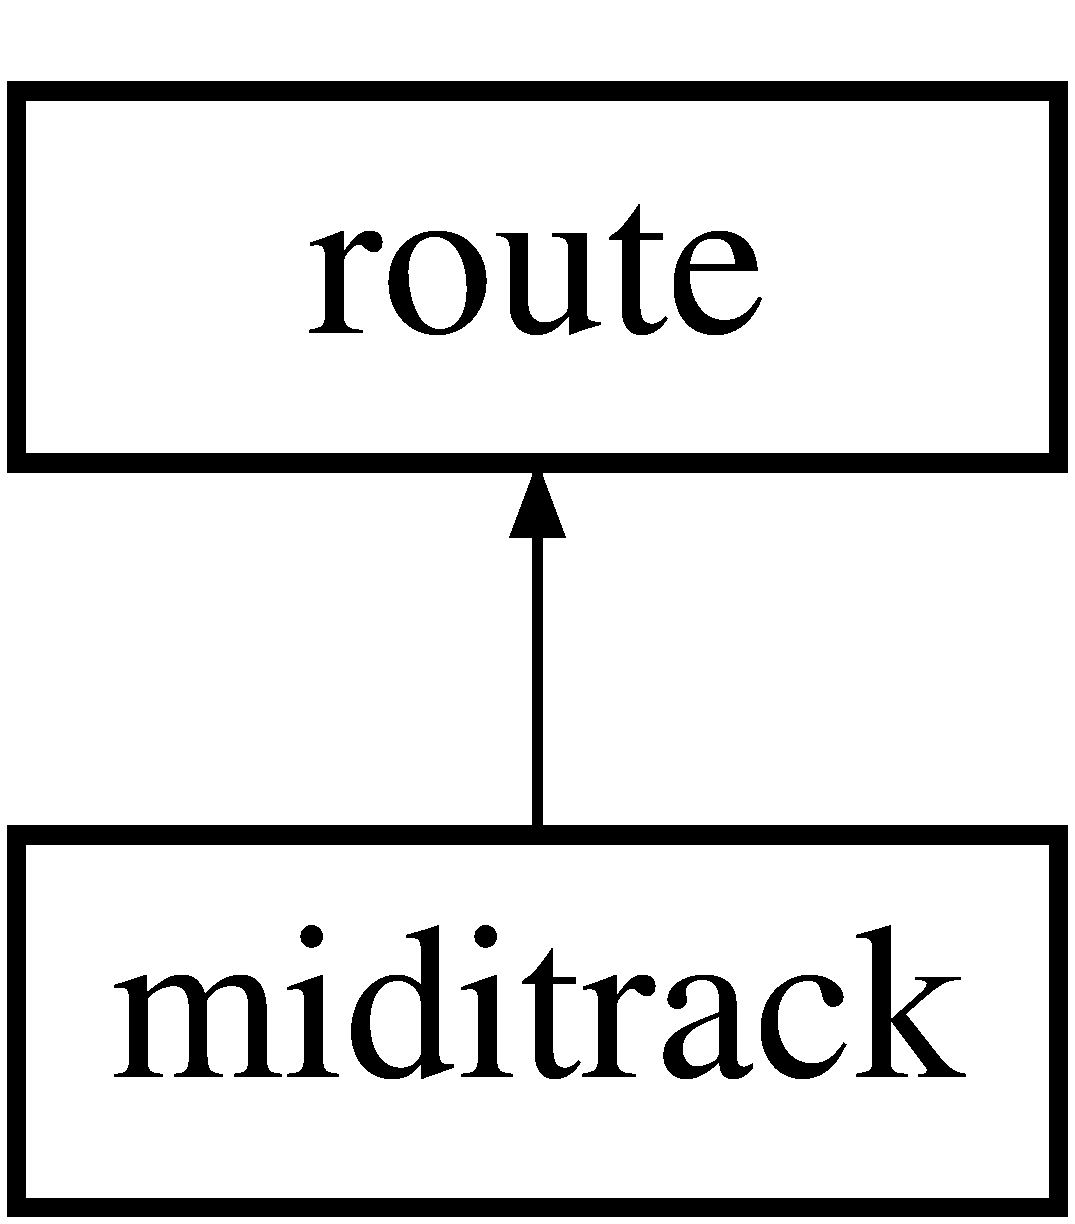
\includegraphics[height=2.000000cm]{classmiditrack}
\end{center}
\end{figure}
\subsection*{Additional Inherited Members}


The documentation for this class was generated from the following files\+:\begin{DoxyCompactItemize}
\item 
src/miditrack.\+h\item 
src/miditrack.\+cpp\end{DoxyCompactItemize}

\hypertarget{classroute}{}\section{route Class Reference}
\label{classroute}\index{route@{route}}
Inheritance diagram for route\+:\begin{figure}[H]
\begin{center}
\leavevmode
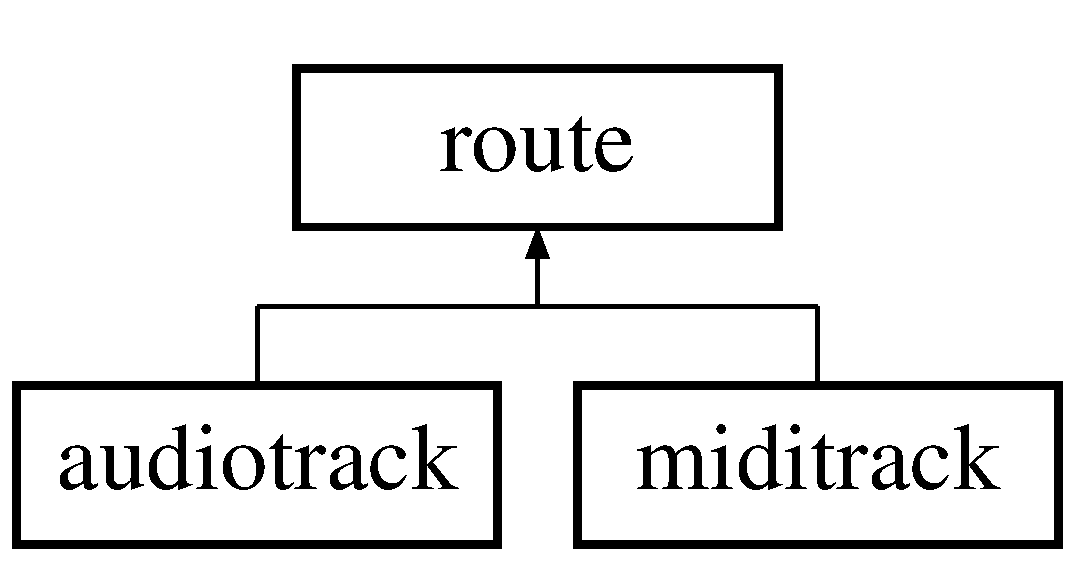
\includegraphics[height=2.000000cm]{classroute}
\end{center}
\end{figure}
\subsection*{Public Member Functions}
\begin{DoxyCompactItemize}
\item 
\mbox{\Hypertarget{classroute_a3de24b4c9f71cd486d46fb6c39a6778d}\label{classroute_a3de24b4c9f71cd486d46fb6c39a6778d}} 
{\bfseries route} (\mbox{\hyperlink{classhandshake}{handshake}} $\ast$hs)
\item 
\mbox{\Hypertarget{classroute_a1b95fb2ceb9751062f3e1d28cbd485b2}\label{classroute_a1b95fb2ceb9751062f3e1d28cbd485b2}} 
{\bfseries route} (std\+::string track\+\_\+name)
\item 
\mbox{\Hypertarget{classroute_ab5d810362212e62f86599b1d80869d43}\label{classroute_ab5d810362212e62f86599b1d80869d43}} 
jack\+\_\+port\+\_\+t $\ast$ \mbox{\hyperlink{classroute_ab5d810362212e62f86599b1d80869d43}{get\+\_\+input\+\_\+port}} ()
\begin{DoxyCompactList}\small\item\em $\ast$\+E\+R\+A\+SE \end{DoxyCompactList}\item 
\mbox{\Hypertarget{classroute_a538c5077d4ff9531a4e905058f278707}\label{classroute_a538c5077d4ff9531a4e905058f278707}} 
jack\+\_\+port\+\_\+t $\ast$ {\bfseries get\+\_\+output\+\_\+port\+\_\+left} ()
\item 
\mbox{\Hypertarget{classroute_a2115b3e03c972f9b8f13cbe91fe0d3bc}\label{classroute_a2115b3e03c972f9b8f13cbe91fe0d3bc}} 
jack\+\_\+port\+\_\+t $\ast$ {\bfseries get\+\_\+output\+\_\+port\+\_\+right} ()
\item 
\mbox{\Hypertarget{classroute_a61f72ad6ee6c070cc207e009f36742a7}\label{classroute_a61f72ad6ee6c070cc207e009f36742a7}} 
void {\bfseries add\+\_\+input} (\mbox{\hyperlink{classhandshake}{handshake}} $\ast$hs)
\item 
\mbox{\Hypertarget{classroute_a66155aecc5f4cb56ff0f365e9c9574d6}\label{classroute_a66155aecc5f4cb56ff0f365e9c9574d6}} 
void {\bfseries add\+\_\+stereo} (\mbox{\hyperlink{classhandshake}{handshake}} $\ast$hs)
\item 
\mbox{\Hypertarget{classroute_a5ea3de9bc26a7b68a9236287e24ce5f1}\label{classroute_a5ea3de9bc26a7b68a9236287e24ce5f1}} 
void {\bfseries add\+\_\+mono} (\mbox{\hyperlink{classhandshake}{handshake}} $\ast$hs)
\item 
\mbox{\Hypertarget{classroute_a72c9ffccca230d286f6e5207dc6b2600}\label{classroute_a72c9ffccca230d286f6e5207dc6b2600}} 
void {\bfseries mute\+\_\+input\+\_\+port} (\mbox{\hyperlink{classhandshake}{handshake}} $\ast$hs)
\item 
\mbox{\Hypertarget{classroute_ac0fa1845cd1c6870e97043c8e1673daa}\label{classroute_ac0fa1845cd1c6870e97043c8e1673daa}} 
void {\bfseries mute\+\_\+stereo\+\_\+port} (\mbox{\hyperlink{classhandshake}{handshake}} $\ast$hs)
\item 
\mbox{\Hypertarget{classroute_a7e7951e060314418b99a844e69ac6ad0}\label{classroute_a7e7951e060314418b99a844e69ac6ad0}} 
void {\bfseries mute\+\_\+mono\+\_\+port} (\mbox{\hyperlink{classhandshake}{handshake}} $\ast$hs)
\item 
\mbox{\Hypertarget{classroute_a14034d6bb5397434136b7cec456ec29d}\label{classroute_a14034d6bb5397434136b7cec456ec29d}} 
void {\bfseries unmute\+\_\+input\+\_\+port} (\mbox{\hyperlink{classhandshake}{handshake}} $\ast$hs)
\item 
\mbox{\Hypertarget{classroute_a0044cc75e5b0eb3f0cfd9c5e62464db8}\label{classroute_a0044cc75e5b0eb3f0cfd9c5e62464db8}} 
void {\bfseries unmute\+\_\+stereo\+\_\+port} (\mbox{\hyperlink{classhandshake}{handshake}} $\ast$hs)
\item 
\mbox{\Hypertarget{classroute_a27bb2f9a0409464f18f73d0ec27b89cd}\label{classroute_a27bb2f9a0409464f18f73d0ec27b89cd}} 
void {\bfseries unmute\+\_\+mono\+\_\+port} (\mbox{\hyperlink{classhandshake}{handshake}} $\ast$hs)
\item 
\mbox{\Hypertarget{classroute_ac1469913cf5f5563a4048df21b111def}\label{classroute_ac1469913cf5f5563a4048df21b111def}} 
void {\bfseries connect\+\_\+all} (\mbox{\hyperlink{classhandshake}{handshake}} $\ast$hs)
\end{DoxyCompactItemize}
\subsection*{Protected Member Functions}
\begin{DoxyCompactItemize}
\item 
\mbox{\Hypertarget{classroute_ae97fe2c45c8d34d6c9d2fbb15f533779}\label{classroute_ae97fe2c45c8d34d6c9d2fbb15f533779}} 
void {\bfseries set\+\_\+routename} (std\+::string routename)
\item 
\mbox{\Hypertarget{classroute_af94e9f62d745063a1e4eb374efff2c32}\label{classroute_af94e9f62d745063a1e4eb374efff2c32}} 
void {\bfseries set\+\_\+portnames} (\mbox{\hyperlink{classhandshake}{handshake}} $\ast$hs)
\item 
\mbox{\Hypertarget{classroute_a0fd630600c37944b7b161e60d5e3c320}\label{classroute_a0fd630600c37944b7b161e60d5e3c320}} 
\mbox{\hyperlink{structtrack__port}{track\+\_\+port}} {\bfseries get\+\_\+track\+\_\+ports} ()
\end{DoxyCompactItemize}


The documentation for this class was generated from the following files\+:\begin{DoxyCompactItemize}
\item 
src/route.\+h\item 
src/route.\+cpp\end{DoxyCompactItemize}

\hypertarget{classsession}{}\section{session Class Reference}
\label{classsession}\index{session@{session}}
\subsection*{Public Member Functions}
\begin{DoxyCompactItemize}
\item 
\mbox{\Hypertarget{classsession_ac47d0baf384a8643d288b65b8a41403a}\label{classsession_ac47d0baf384a8643d288b65b8a41403a}} 
{\bfseries session} (const char $\ast$session\+\_\+name)
\item 
\mbox{\Hypertarget{classsession_a1cac142e82111a5560b8bd7f751d90cd}\label{classsession_a1cac142e82111a5560b8bd7f751d90cd}} 
void {\bfseries save} ()
\item 
\mbox{\Hypertarget{classsession_a19927891dbba8c1e0af4246437cefd2b}\label{classsession_a19927891dbba8c1e0af4246437cefd2b}} 
void {\bfseries load} ()
\item 
\mbox{\Hypertarget{classsession_a9bf140b2437977c59f0e51662f7393ee}\label{classsession_a9bf140b2437977c59f0e51662f7393ee}} 
void {\bfseries wipe} ()
\item 
\mbox{\Hypertarget{classsession_a26a7e5d3911fa8b33660fe40d1d07dfc}\label{classsession_a26a7e5d3911fa8b33660fe40d1d07dfc}} 
\mbox{\hyperlink{classchannel}{channel}} $\ast$ {\bfseries get\+\_\+channel} ()
\end{DoxyCompactItemize}


The documentation for this class was generated from the following files\+:\begin{DoxyCompactItemize}
\item 
src/session.\+h\item 
src/session.\+cpp\end{DoxyCompactItemize}

\hypertarget{classtrack}{}\section{track Class Reference}
\label{classtrack}\index{track@{track}}
\subsection*{Public Member Functions}
\begin{DoxyCompactItemize}
\item 
\mbox{\Hypertarget{classtrack_a73b8004e9a8b81338ee652049e74f81c}\label{classtrack_a73b8004e9a8b81338ee652049e74f81c}} 
jack\+\_\+port\+\_\+t $\ast$ {\bfseries get\+\_\+input\+\_\+port} ()
\item 
\mbox{\Hypertarget{classtrack_ae5e47dd339c9d8aae5541b64ff7be99f}\label{classtrack_ae5e47dd339c9d8aae5541b64ff7be99f}} 
jack\+\_\+port\+\_\+t $\ast$ {\bfseries get\+\_\+output\+\_\+port\+\_\+left} ()
\item 
\mbox{\Hypertarget{classtrack_ad015bc9df6d1b44ae54a6d694b5eb3f2}\label{classtrack_ad015bc9df6d1b44ae54a6d694b5eb3f2}} 
jack\+\_\+port\+\_\+t $\ast$ {\bfseries get\+\_\+output\+\_\+port\+\_\+right} ()
\item 
\mbox{\Hypertarget{classtrack_ab9fa8e83130174346e96071751109b11}\label{classtrack_ab9fa8e83130174346e96071751109b11}} 
jack\+\_\+port\+\_\+t $\ast$ {\bfseries get\+\_\+mono\+\_\+port} ()
\item 
\mbox{\Hypertarget{classtrack_a459b2d8e7cd388a2170e8369ba4f267c}\label{classtrack_a459b2d8e7cd388a2170e8369ba4f267c}} 
void {\bfseries register\+\_\+input\+\_\+ports} (jack\+\_\+client\+\_\+t $\ast$client, unsigned long flag)
\item 
\mbox{\Hypertarget{classtrack_a1b34b6eac8eb1c09673b8c750f61b94f}\label{classtrack_a1b34b6eac8eb1c09673b8c750f61b94f}} 
void {\bfseries register\+\_\+output\+\_\+ports} (jack\+\_\+client\+\_\+t $\ast$client, unsigned long flag)
\item 
\mbox{\Hypertarget{classtrack_aababee8291bfeaf41a31caca35b499fe}\label{classtrack_aababee8291bfeaf41a31caca35b499fe}} 
void {\bfseries mute} (jack\+\_\+client\+\_\+t $\ast$client)
\item 
\mbox{\Hypertarget{classtrack_a2f0074c13cebe0a60bf31af31a9dc260}\label{classtrack_a2f0074c13cebe0a60bf31af31a9dc260}} 
void {\bfseries playback} ()
\item 
\mbox{\Hypertarget{classtrack_aabf7c10f62e25a3d6a7e6bbed4570531}\label{classtrack_aabf7c10f62e25a3d6a7e6bbed4570531}} 
void {\bfseries record} ()
\item 
\mbox{\Hypertarget{classtrack_af118a033f9bfb048c5da9486bd85a643}\label{classtrack_af118a033f9bfb048c5da9486bd85a643}} 
void {\bfseries overdub} ()
\item 
\mbox{\Hypertarget{classtrack_a6b2cea1fdb0f55b67bf0e2e0777bcb9f}\label{classtrack_a6b2cea1fdb0f55b67bf0e2e0777bcb9f}} 
int {\bfseries monitor} (uint32\+\_\+t nframes)
\item 
\mbox{\Hypertarget{classtrack_a645137cd6b283eb3f2f5a72c1eea8c74}\label{classtrack_a645137cd6b283eb3f2f5a72c1eea8c74}} 
const char $\ast$ {\bfseries get\+\_\+uniqname} ()
\item 
\mbox{\Hypertarget{classtrack_a570b552f2a08daaff3fe0ba993f88ab2}\label{classtrack_a570b552f2a08daaff3fe0ba993f88ab2}} 
void {\bfseries set\+\_\+uniqname} ()
\item 
\mbox{\Hypertarget{classtrack_aeb12911b71eb76a226cf4d3750fa70d1}\label{classtrack_aeb12911b71eb76a226cf4d3750fa70d1}} 
void {\bfseries mute\+\_\+input\+\_\+ports} (jack\+\_\+client\+\_\+t $\ast$client)
\item 
\mbox{\Hypertarget{classtrack_af6a0dfeed9dd6551d228631a9acac33c}\label{classtrack_af6a0dfeed9dd6551d228631a9acac33c}} 
void {\bfseries mute\+\_\+output\+\_\+ports} (jack\+\_\+client\+\_\+t $\ast$client)
\end{DoxyCompactItemize}
\subsection*{Public Attributes}
\begin{DoxyCompactItemize}
\item 
\mbox{\Hypertarget{classtrack_adceeb14b636b259fc4c06f5d67ffaf81}\label{classtrack_adceeb14b636b259fc4c06f5d67ffaf81}} 
\mbox{\hyperlink{structtrack__port}{track\+\_\+port}} {\bfseries tp}
\item 
\mbox{\Hypertarget{classtrack_a239c9e283c7ecae2bbe5bbc16a89eec7}\label{classtrack_a239c9e283c7ecae2bbe5bbc16a89eec7}} 
const char $\ast$ {\bfseries uniqname}
\end{DoxyCompactItemize}


The documentation for this class was generated from the following files\+:\begin{DoxyCompactItemize}
\item 
src/track.\+h\item 
src/track.\+cpp\end{DoxyCompactItemize}

\hypertarget{structtrack__port}{}\section{track\+\_\+port Struct Reference}
\label{structtrack__port}\index{track\+\_\+port@{track\+\_\+port}}
\subsection*{Public Attributes}
\begin{DoxyCompactItemize}
\item 
\mbox{\Hypertarget{structtrack__port_a1d925d57307d6b17c503ced4aa99a8bd}\label{structtrack__port_a1d925d57307d6b17c503ced4aa99a8bd}} 
jack\+\_\+port\+\_\+t $\ast$ {\bfseries input\+\_\+port}
\item 
\mbox{\Hypertarget{structtrack__port_a32201649f5f0fe8cb52a1a05f4292f94}\label{structtrack__port_a32201649f5f0fe8cb52a1a05f4292f94}} 
jack\+\_\+port\+\_\+t $\ast$ {\bfseries output\+\_\+port\+\_\+left}
\item 
\mbox{\Hypertarget{structtrack__port_a5bf5d29bcc3001f5b69350f14d54da6e}\label{structtrack__port_a5bf5d29bcc3001f5b69350f14d54da6e}} 
jack\+\_\+port\+\_\+t $\ast$ {\bfseries output\+\_\+port\+\_\+right}
\item 
\mbox{\Hypertarget{structtrack__port_a9e1a7657a8e1b3852c76c1d504ca8e68}\label{structtrack__port_a9e1a7657a8e1b3852c76c1d504ca8e68}} 
jack\+\_\+port\+\_\+t $\ast$ {\bfseries output\+\_\+port\+\_\+mono}
\end{DoxyCompactItemize}


The documentation for this struct was generated from the following file\+:\begin{DoxyCompactItemize}
\item 
src/route.\+h\end{DoxyCompactItemize}

%--- End generated contents ---

% Index
\backmatter
\newpage
\phantomsection
\clearemptydoublepage
\addcontentsline{toc}{chapter}{Index}
\printindex

\end{document}
